% ------------------------------------------------------------
% DO NOT CHANGE: BEGIN
% ------------------------------------------------------------

\usepackage[utf8]{inputenc}  
\usepackage[T1]{fontenc}  
\usepackage{lmodern}
\usepackage[english]{babel}
\usepackage{fancybox}
\usepackage{listings}
\usepackage{color}
\usepackage{graphicx,subfigure}
\usepackage[titletoc]{appendix}
\usepackage{float} % figures flottantes 
\usepackage{here} % figures flottantes
\usepackage{url}
\usepackage{enumitem}
\setlist[itemize]{noitemsep, nolistsep}
\setlist[enumerate]{noitemsep, nolistsep}
\usepackage{xcolor}
\usepackage[colorlinks=true]{hyperref}
\usepackage{tabularx}
\usepackage{minted}
\usepackage{amsmath}
\usepackage[skins,breakable]{tcolorbox}

% --------------------------------------------------------------
% Title
% --------------------------------------------------------------
\makeatletter
\newcommand\maintitle[1]{
    \quitvmode
    \hb@xt@\linewidth{
        \dimen@=1ex
        \advance\dimen@-2pt
        \leaders\hrule \@height1ex \@depth-\dimen@\hfill
        \enskip
        \textbf{#1}
        \enskip
        \leaders\hrule \@height1ex \@depth-\dimen@\hfill
    }
}
\makeatother

% --------------------------------------------------------------
% Some parameters
% --------------------------------------------------------------
\oddsidemargin =0 mm
\topmargin = -10 mm
\footskip = 20mm
\textheight = 240 mm 
\textwidth = 160mm

% --------------------------------------------------------------
% Q&A environments
% --------------------------------------------------------------

\newcommand{\emptyquestion}{Please fill this space with your question.}

\newcommand{\emptyanswer}{Please fill this space with your answer.}

\newcounter{question}

\definecolor{question_color}{RGB}{181,124,64}
\definecolor{question_color_fill}{RGB}{252,248,227}

\newcommand{\thequestionref}{No reference}

\makeatletter
\newenvironment{question}[1]
{
\refstepcounter{question}
\def\@currentlabel{{#1}}
\label{ref-question-\thequestion}
\addcontentsline{toc}{subsection}{{#1}}
\noindent
\begin{tcolorbox}[
    colframe=question_color,
    colback=question_color_fill,
    coltitle=question_color_fill,  
    title=\centering\textbf{Question #1:},
    breakable,
    width=\textwidth]
}
{   \end{tcolorbox}
}
\makeatother

\newenvironment{answer}
{
\noindent
{
\hypersetup{allcolors=question_color}
\flushleft
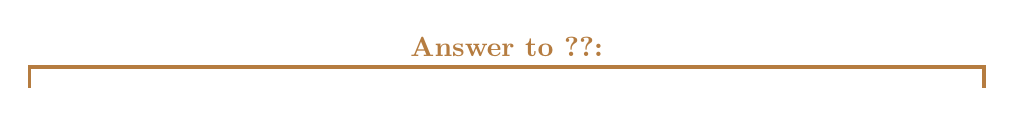
\begin{tikzpicture}
    \draw[very thick,question_color] (0,0) -- ++(0,+7.5pt)
    -- ++(\textwidth,0) node[midway,above] {\textbf{Answer to \ref{ref-question-\thequestion}:}}
    -- ++(0,-7.5pt);
\end{tikzpicture}
\vspace{-.3cm}
}
\begin{tcolorbox}[
    blanker,
    width=\textwidth,
    breakable]
}
{   \end{tcolorbox}
\vspace{-.4cm}
\flushleft

\begin{tikzpicture}
    \draw[very thick,question_color] (0,0) -- ++(0,-7.5pt)
    -- ++(\textwidth,0)
    -- ++(0,+7.5pt);
\end{tikzpicture}
}

\usepackage{tikz}

% --------------------------------------------------------------
% Code environments
% --------------------------------------------------------------
\usemintedstyle{borland}
\providecommand*{\listingautorefname}{Listing}

\newenvironment{python}
{\VerbatimEnvironment
\begin{minted}[
linenos,
% fontfamily=courier,
fontsize=\normalsize,
xleftmargin=21pt,
]{python}}
{\end{minted}}

\newcommand\py[1]{\mintinline{python}{#1}}

\newcommand\la[1]{\mintinline{latex}{#1}}

% --------------------------------------------------------------
% CELL environments
% --------------------------------------------------------------

\newcounter{cell}

\definecolor{cell_color}{RGB}{7,128,164}
\definecolor{cell_color_fill}{RGB}{247,247,247}

\newcommand{\thecellref}{No reference}

\makeatletter
\newenvironment{cell}[1]
{
\refstepcounter{cell}
\def\@currentlabel{{#1}}
\label{ref-cell-\thecell}
\addcontentsline{toc}{subsection}{\texttt{CELL N$^{\circ}${#1}}}
\noindent
\begin{tcolorbox}[
    colframe=cell_color,
    colback=cell_color_fill,
    coltitle=cell_color_fill,  
    title=\centering\texttt{CELL N$^{\circ}${#1}:},
    breakable,
    width=\textwidth]
}
{   \end{tcolorbox}
}
\makeatother

% ------------------------------------------------------------
% DO NOT CHANGE: END
% ------------------------------------------------------------